\documentclass[13pt, t]{beamer}
% Presento style file
\usepackage{config/presento}

% custom command and packages
% custom packages
\usepackage{textpos}
\setlength{\TPHorizModule}{1cm}
\setlength{\TPVertModule}{1cm}

\newcommand\crule[1][black]{\textcolor{#1}{\rule{2cm}{2cm}}}



\usepackage{color, colortbl}
\setlength{\columnseprule}{0.4pt} 

\title{\Large \hspace{-0.5cm} Phonetic fieldwork and experiments with the \texttt{phonfieldwork} package for R}
\author[shortname]{George Moroz}
\institute[shortinst]{Linguistic Convergence Laboratory, NRU HSE, Moscow, Russia}
\date{\begin{center} {\large 15 November 2019} \bigskip \\ {NRU HSE, School of linguistics, Moscow}\\ \vfill Presentation is available here: {\large \href{https://tinyurl.com/yzd2yjr5}{tinyurl.com/yzd2yjr5} \hfill 
\includegraphics[height = 2.5cm]{images/01_qrcode}} \end{center}}

\begin{document}

\begin{frame}[plain]
\maketitle
\end{frame}

\begin{frame}{Most phonetic research consists of the following steps:}
\begin{enumerate}
\item Formulate a research question. Think of what kind of data is necessary to answer this question, what is the appropriate amount of data, what kind of annotation you will do, what kind of statistical models and visualizations you will use, etc.
\item Create a list of stimuli.
\item Elicite list of stimuli from speakers who signed an Informed Consent statement, agreeing to participate in the experiment to be recorded on audio and/or video.
\item Annotate the collected data.
\item Extract the information from annotated data.
\item Create visualizations and evaluate your statistical models.
\item Report your results.
\item Publish your data. \pause
\end{enumerate}
The \texttt{phonfieldwork} package is created for helping with items 3, partially with 4, and 5 and 8.
\end{frame}

\begin{frame}{Why/when do you need the \texttt{phonfieldwork} package?}
These ideal plan hides some technical subtasks:
\begin{itemize}
\item creating a presentation for elicitation task
\item renaming and concatenating multiple sound files recorded during a session
\item automatic annotation in Praat TextGrids {\small \citep{boersma19}}
\item creating a searchable \texttt{.html} table with annotations, spectrograms and ability to hear sound
\item converting multiple formats (Praat, ELAN \citep{brugman04} and EXMARaLDA \citep{schmidt09}) \pause
\end{itemize}
\vfill
All of these tasks can be solved by a mixture of different tools:
\begin{itemize}
\item any programming language can handle automatic  file renaming
\item Praat contains scripts for concatenating and renaming files
\end{itemize}
\pause
\vfill
\texttt{phonfieldwork} provides a functionality that will make it easier to solve those tasks independently of any additional tools. You can also compare the functionality with other R packages:\\ \texttt{rPraat} \citep{borzil16} and \texttt{textgRid} \citep{reidy16}, \texttt{pympi} \citep{lubbers13}
\end{frame}

\begin{frame}{Philosophy of the \texttt{phonfieldwork} package}
\begin{itemize}
\item each stimulus as a separate file
\item researcher carefully listens to consultants to make sure that they are producing the kind of speech they wanted
\item in case a speaker does not produce three clear repetitions, researcher ask them to repeat the task
\end{itemize}

There are some phoneticians who prefer to record everything, for language documentation purposes. I think that should be a separate task. If you insist on recording everything, it is possible to run two recorders at the same time: one could run during the whole session, while the other is used to produce small audio files. You can also use special software to record your stimuli automatically on a computer (e.g. \texttt{PsychoPy} \citep{peirce19}).
\end{frame}


\framecard[colorblue]{{\color{colorwhite} \Large Let's go through \textbf{phonfieldwork} functionality\pause :\\
\begin{itemize}
\item[\color{colorwhite} $\bullet$] \color{colorwhite} install the package
\item[\color{colorwhite} $\bullet$] \color{colorwhite} create a presentation based on a list of stimuli
\item[\color{colorwhite} $\bullet$] \color{colorwhite} rename collected data
\item[\color{colorwhite} $\bullet$] \color{colorwhite} merge all data together
\item[\color{colorwhite} $\bullet$] \color{colorwhite} automatically annotate your data
\item[\color{colorwhite} $\bullet$] \color{colorwhite} extract annotated fragments
\item[\color{colorwhite} $\bullet$] \color{colorwhite} visualize your data
\item[\color{colorwhite} $\bullet$] \color{colorwhite} create an \textbf{.html} viewer
\item[\color{colorwhite} $\bullet$] \color{colorwhite} cite the package
\end{itemize}

}}

\begin{frame}[fragile]{Install the package}
\begin{itemize}
\item Install the package from CRAN:
\begin{verbatim}
install.packages("phonfieldwork")
\end{verbatim}
\vfill
\item \dots or install it from Github:
\begin{verbatim}
install.packages("devtools")
devtools::install_github("agricolamz/phonfieldwork") 
\end{verbatim} 
\pause \vfill
\item Load the package:
\begin{verbatim}
library("phonfieldwork")
packageVersion("phonfieldwork")

## [1] '0.0.3'
\end{verbatim}


\end{itemize}
\end{frame}

\begin{frame}[fragile]{Create a presentation based on a list of stimuli}
There are several ways to enter information about a list of stimuli into R:
\begin{itemize}
\item listing stimuli with the \texttt{c()}  function inside R
\begin{verbatim}
c("tip", "tap", "top")
[1] "tip" "tap" "top"
\end{verbatim}
\item importing \texttt{.csv} file inside R using the \texttt{read.csv()} function:
\begin{verbatim}
read.csv("my_stimuli_df.csv")
  stimuli vowel
1     tip     ı
2     tap     æ
3     top     ɒ
\end{verbatim}
\item importing data from \texttt{.xls} or \texttt{.xlsx} file inside R using the \texttt{read.csv()} function:
\begin{verbatim}
read.csv("my_stimuli_df.csv")
  stimuli vowel
1     tip     ı
2     tap     æ
3     top     ɒ
\end{verbatim}
\end{itemize}
\end{frame}

\begin{frame}[fragile]{Create a presentation based on a list of stimuli}
\begin{itemize}
\item Now we are ready for creating a presentation for elicitation:
\begin{verbatim}
create_presentation(stimuli = my_stimuli$stimuli,
                    output_file = "first_example",
                    output_dir = getwd()) 
\end{verbatim}
\href{https://agricolamz.github.io/phonfieldwork/first_example.html}{Here} is the result.
\item Here is another example with translations:
\begin{verbatim}
create_presentation(stimuli = my_stimuli$stimuli,
                    translation = c("чаевые", "кран", "верхушка"),
                    output_file = "first_example",
                    output_dir = getwd()) 
\end{verbatim}
\href{https://agricolamz.github.io/phonfieldwork/second_example.html}{Here} is the result.
\end{itemize}
\end{frame}

\begin{frame}[fragile]{Rename collected data}
After collecting data and removing soundfiles with unsuccesful elicitations, one could end up with the following structure:
\begin{verbatim}
## ├── s1
## │   ├── 01.wav
## │   ├── 02.wav
## │   └── 03.wav
## └── s2
##     ├── 01.wav
##     ├── 02.wav
##     └── 03.wav
\end{verbatim}
\end{frame}

\begin{frame}[fragile]{Rename collected data}
Let's rename the files:
\begin{verbatim}
rename_soundfiles(stimuli = my_stimuli$stimuli,
                  prefix = "s1_",
                  path = "s1/")
## ├── s1
## │   ├── backup
## │   │   ├── 01.wav
## │   │   ├── 02.wav
## │   │   └── 03.wav
## │   ├── s1_tap.wav
## │   ├── s1_tip.wav
## │   └── s1_top.wav
## └── s2
##     ├── 01.wav
##     ├── 02.wav
##     └── 03.wav
\end{verbatim}
\end{frame}

\begin{frame}[fragile]{Rename collected data}
\begin{verbatim}
rename_soundfiles(stimuli = my_stimuli$stimuli,
                  prefix = "s2_",
                  suffix = paste0("_", 1:3),
                  path = "s2/",
                  backup = FALSE)
## ├── s1
## │   ├── backup
## │   │   ├── 01.wav
## │   │   ├── 02.wav
## │   │   └── 03.wav
## │   ├── s1_tap.wav
## │   ├── s1_tip.wav
## │   └── s1_top.wav
## └── s2
##     ├── s2_tap_2.wav
##     ├── s2_tip_1.wav
##     └── s2_top_3.wav                  
\end{verbatim}
\end{frame}

\begin{frame}[fragile]{Merge all data together}
\begin{verbatim}
concatenate_soundfiles(file_name = "s1_all",
                       path = "s1/")
## ├── s1
## │   ├── backup
## │   │   ├── 01.wav
## │   │   ├── 02.wav
## │   │   └── 03.wav
## │   ├── s1_all.TextGrid
## │   ├── s1_all.wav
## │   ├── s1_tap.wav
## │   ├── s1_tip.wav
## │   └── s1_top.wav
## └── s2
##     ├── s2_tap_2.wav
##     ├── s2_tip_1.wav
##     └── s2_top_3.wav                       
\end{verbatim}
\end{frame}

\begin{frame}[fragile]{Merge all data together}
Here is how \texttt{s1\_all.TextGrid} and \texttt{s1\_all.wav} look like:
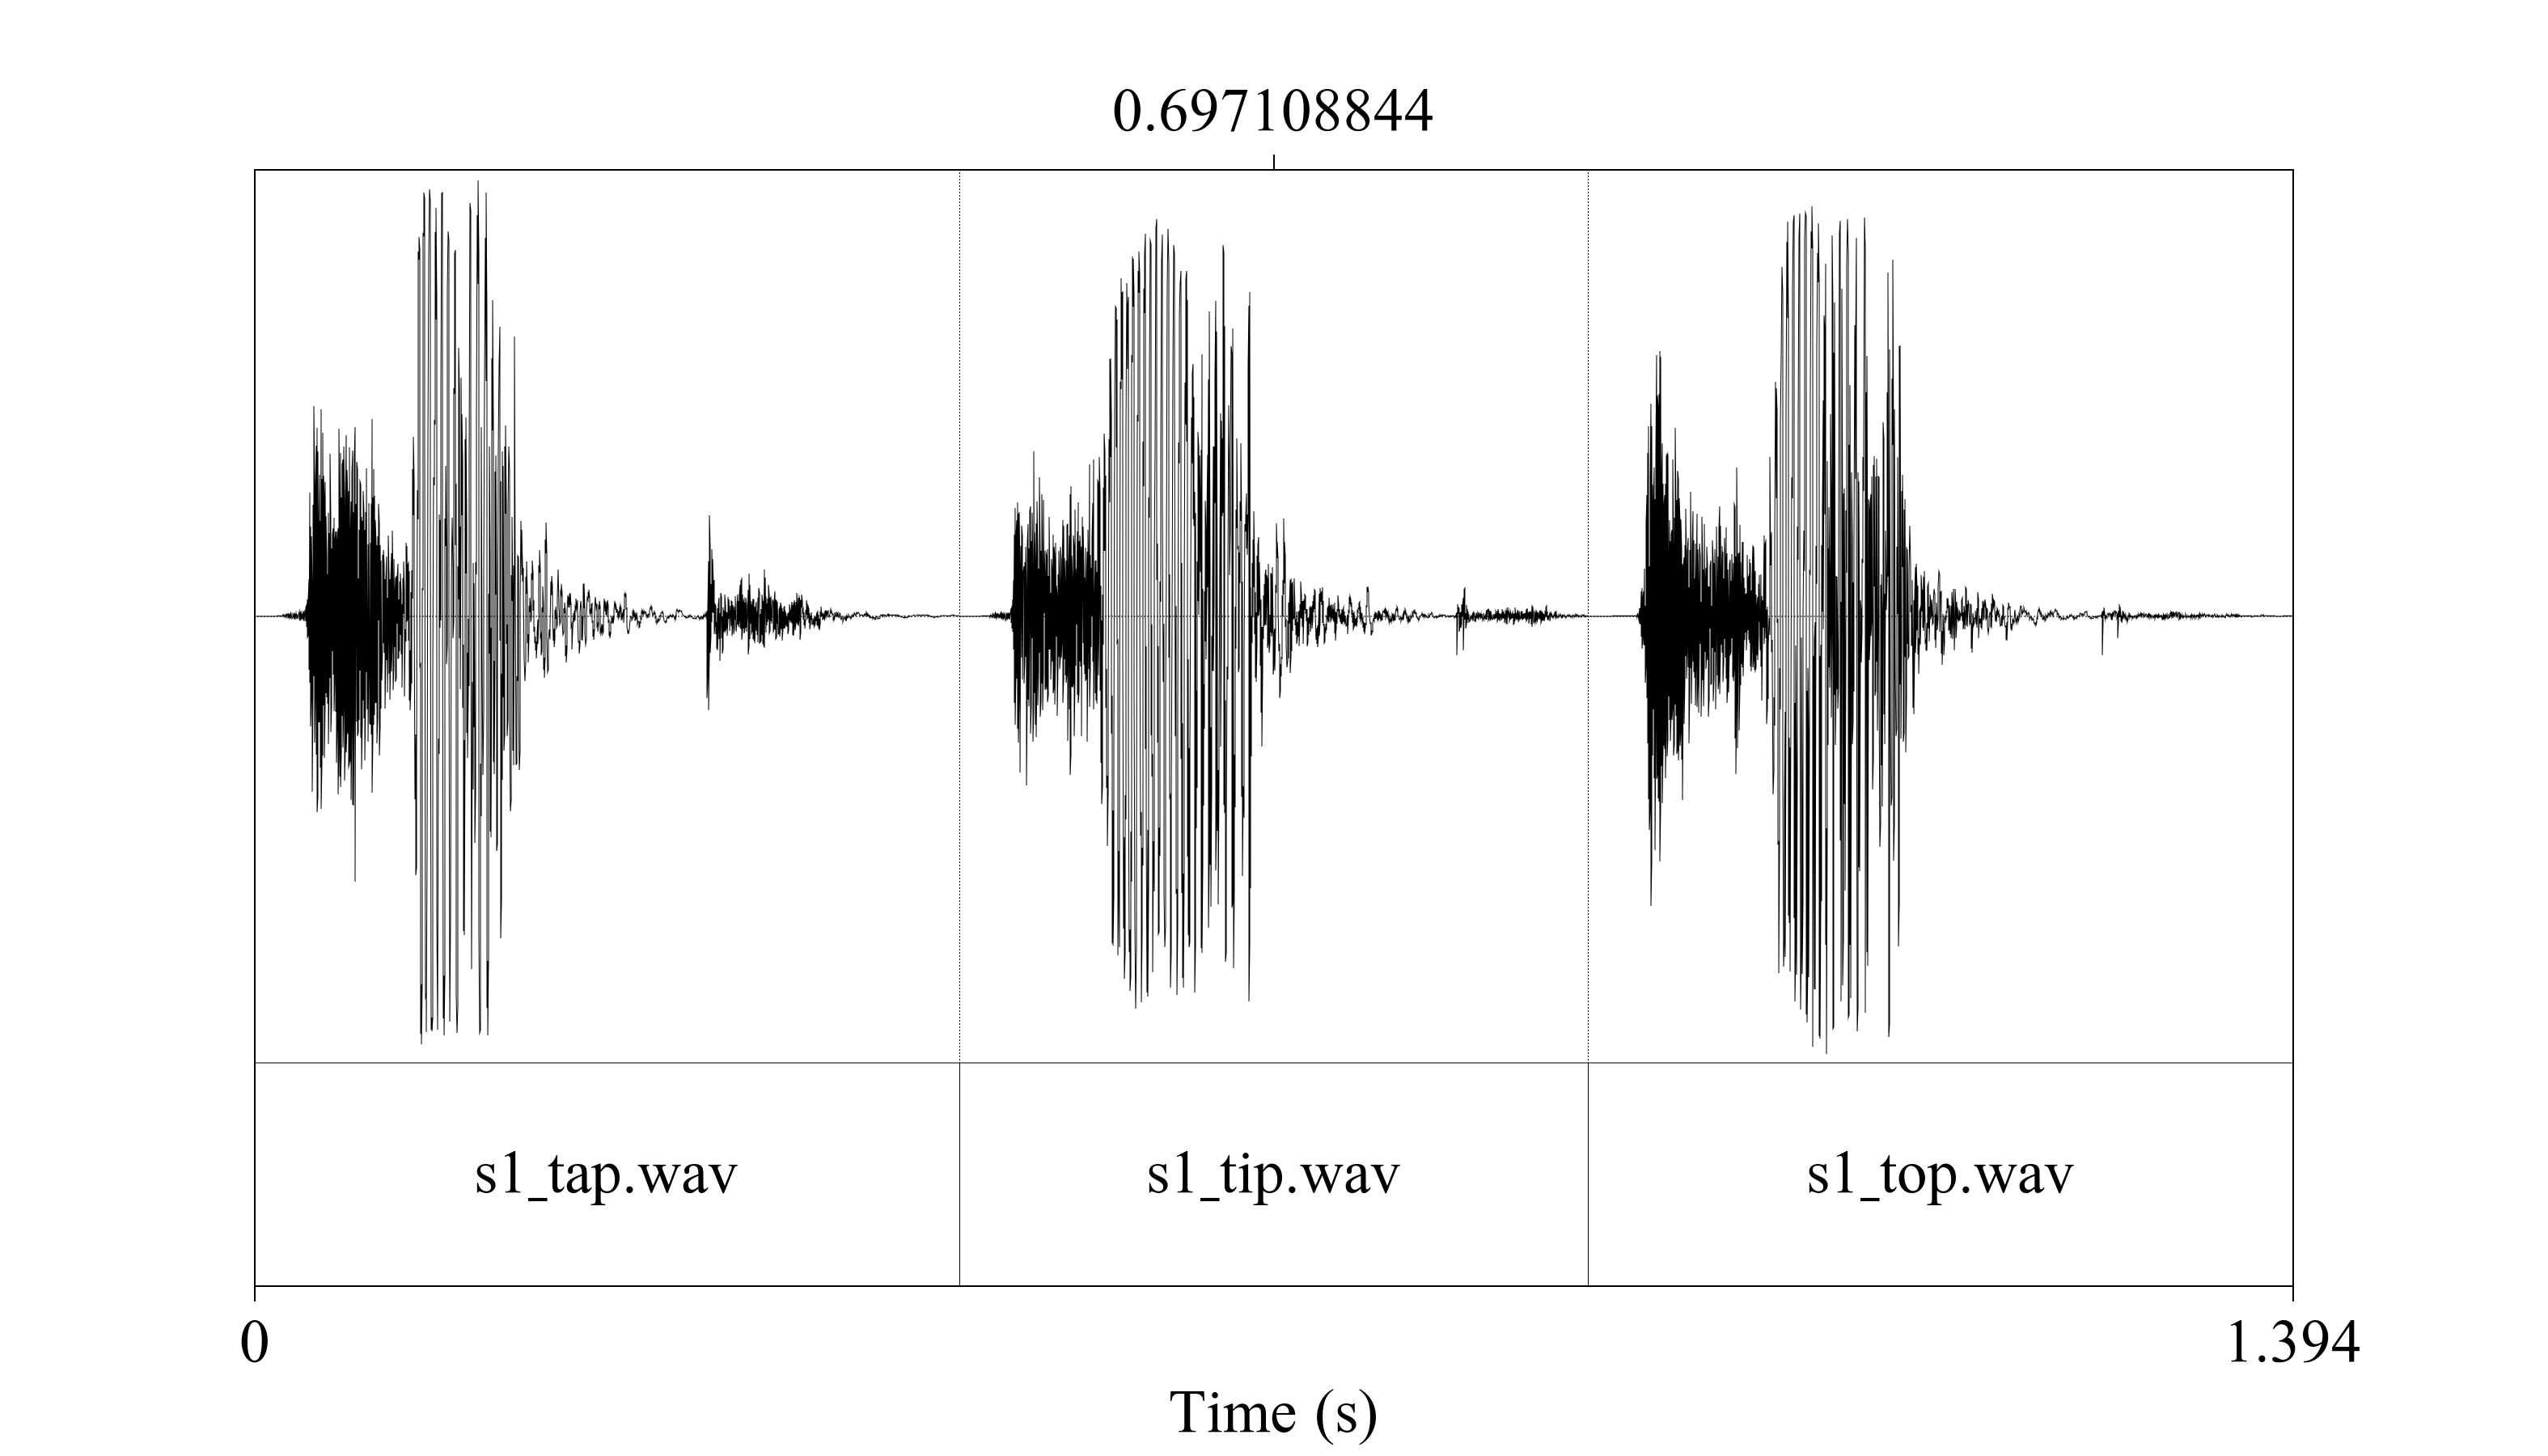
\includegraphics[width=\linewidth]{images/03_concatenate.png}
\end{frame}

\begin{frame}[fragile]{Automatically annotate your data}
\begin{verbatim}
annotate_textgrid(annotation = my_stimuli$stimuli,
                  textgrid = "s1/s1_all.TextGrid")
\end{verbatim}
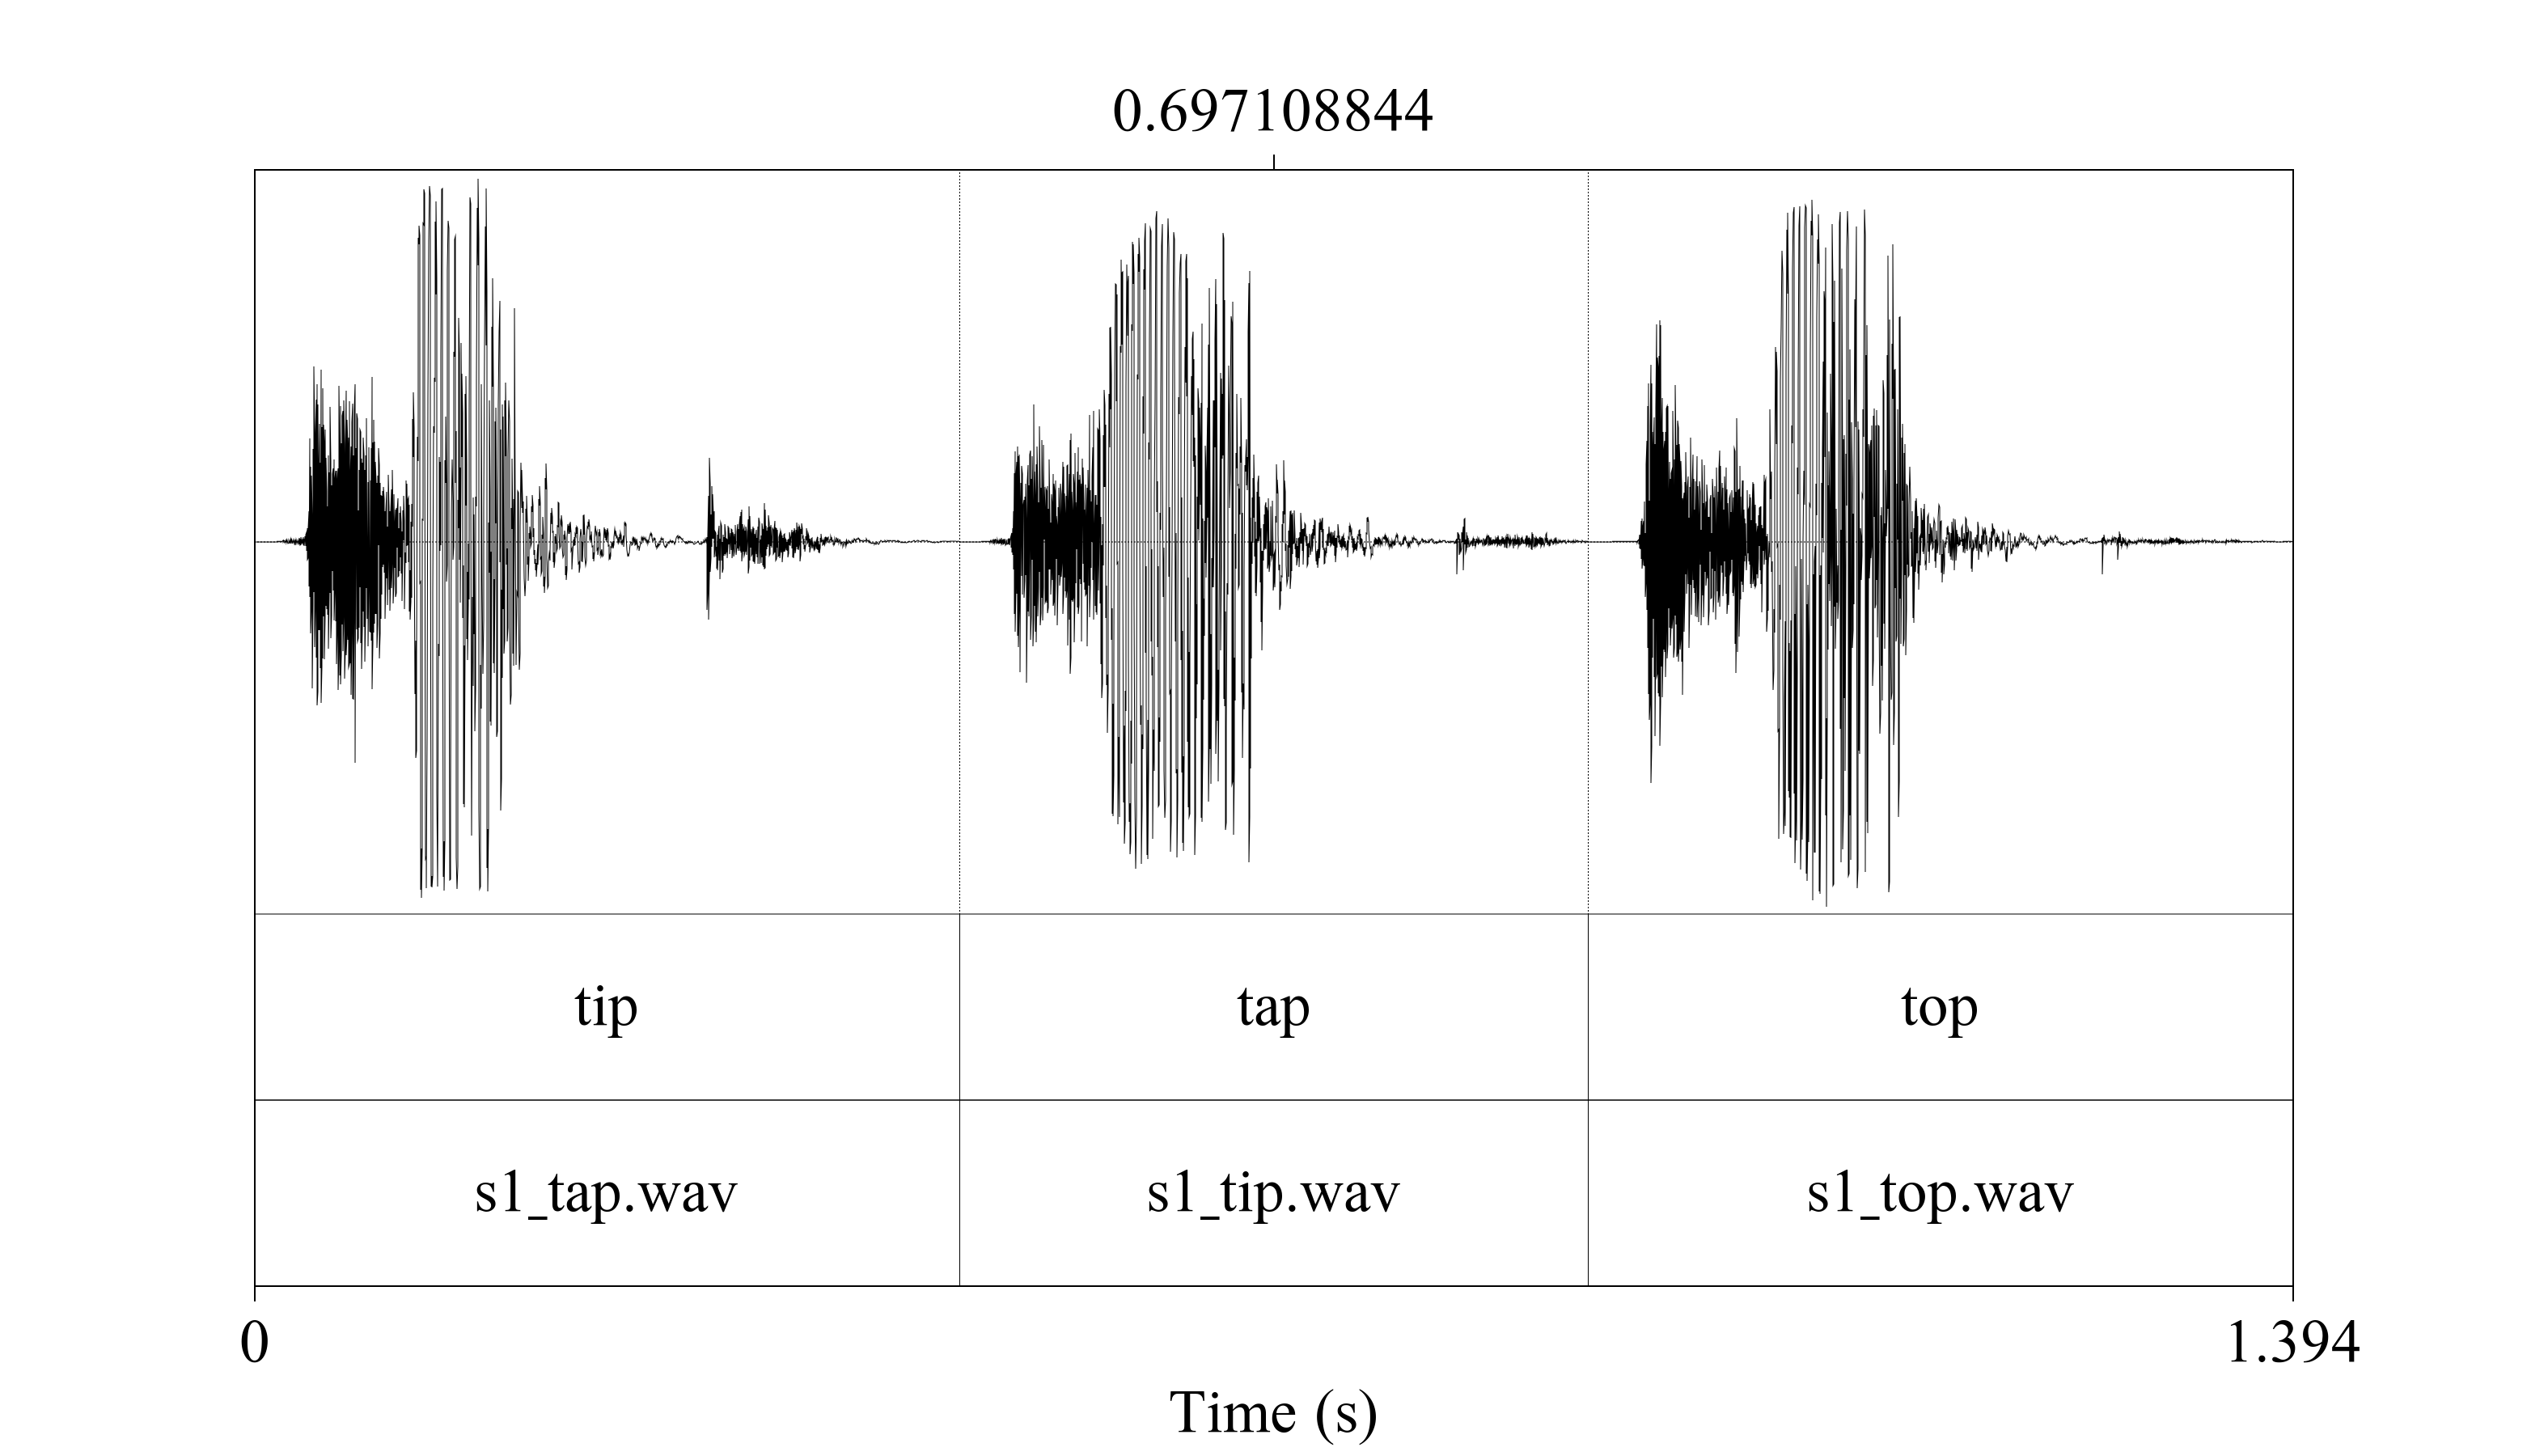
\includegraphics[width=\linewidth]{images/04_annotate.png}
\end{frame}

\begin{frame}[fragile]{Automatically annotate your data}
Imagine that someone manually annotated each vowel in the recording, so the \texttt{.TextGrid} will look as follows:
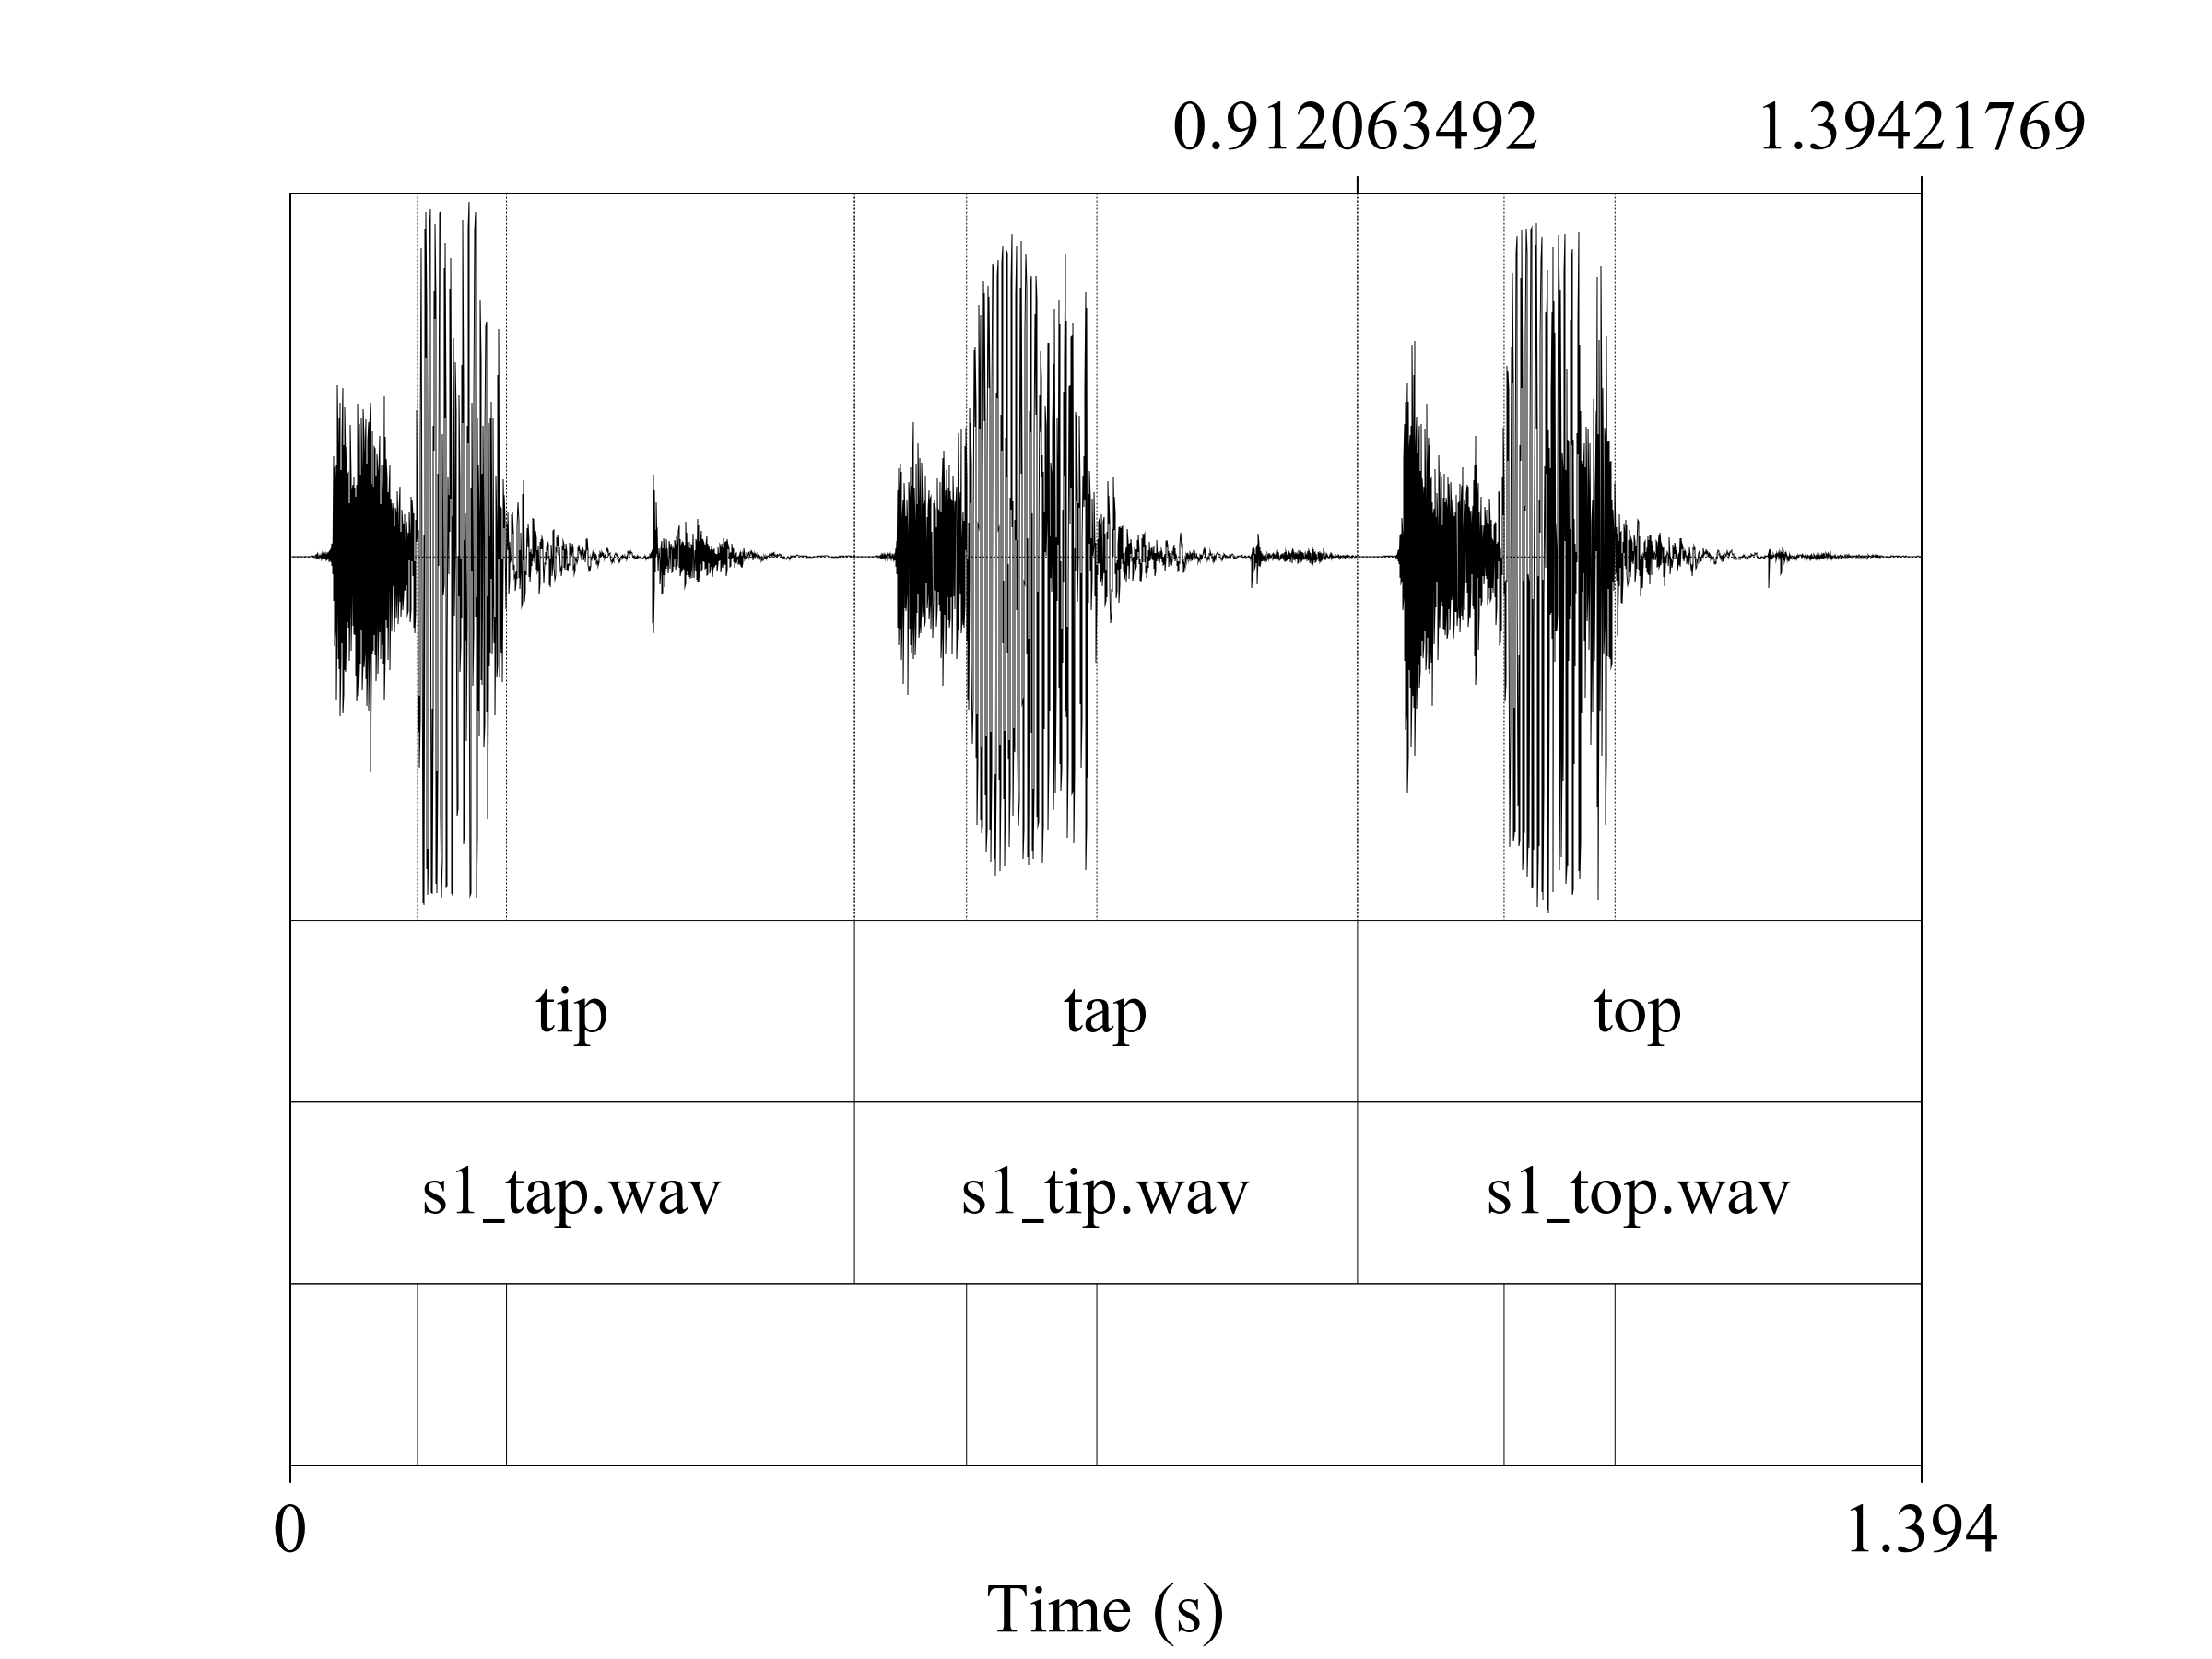
\includegraphics[width=0.92\linewidth]{images/05_annotate.png}
\end{frame}

\begin{frame}[fragile]{Automatically annotate your data}
\begin{verbatim}
annotate_textgrid(annotation = my_stimuli$vowel,
                  textgrid = "s1/s1_all.TextGrid",
                  each = 2,
                  tier = 3, 
                  backup = FALSE)
\end{verbatim}
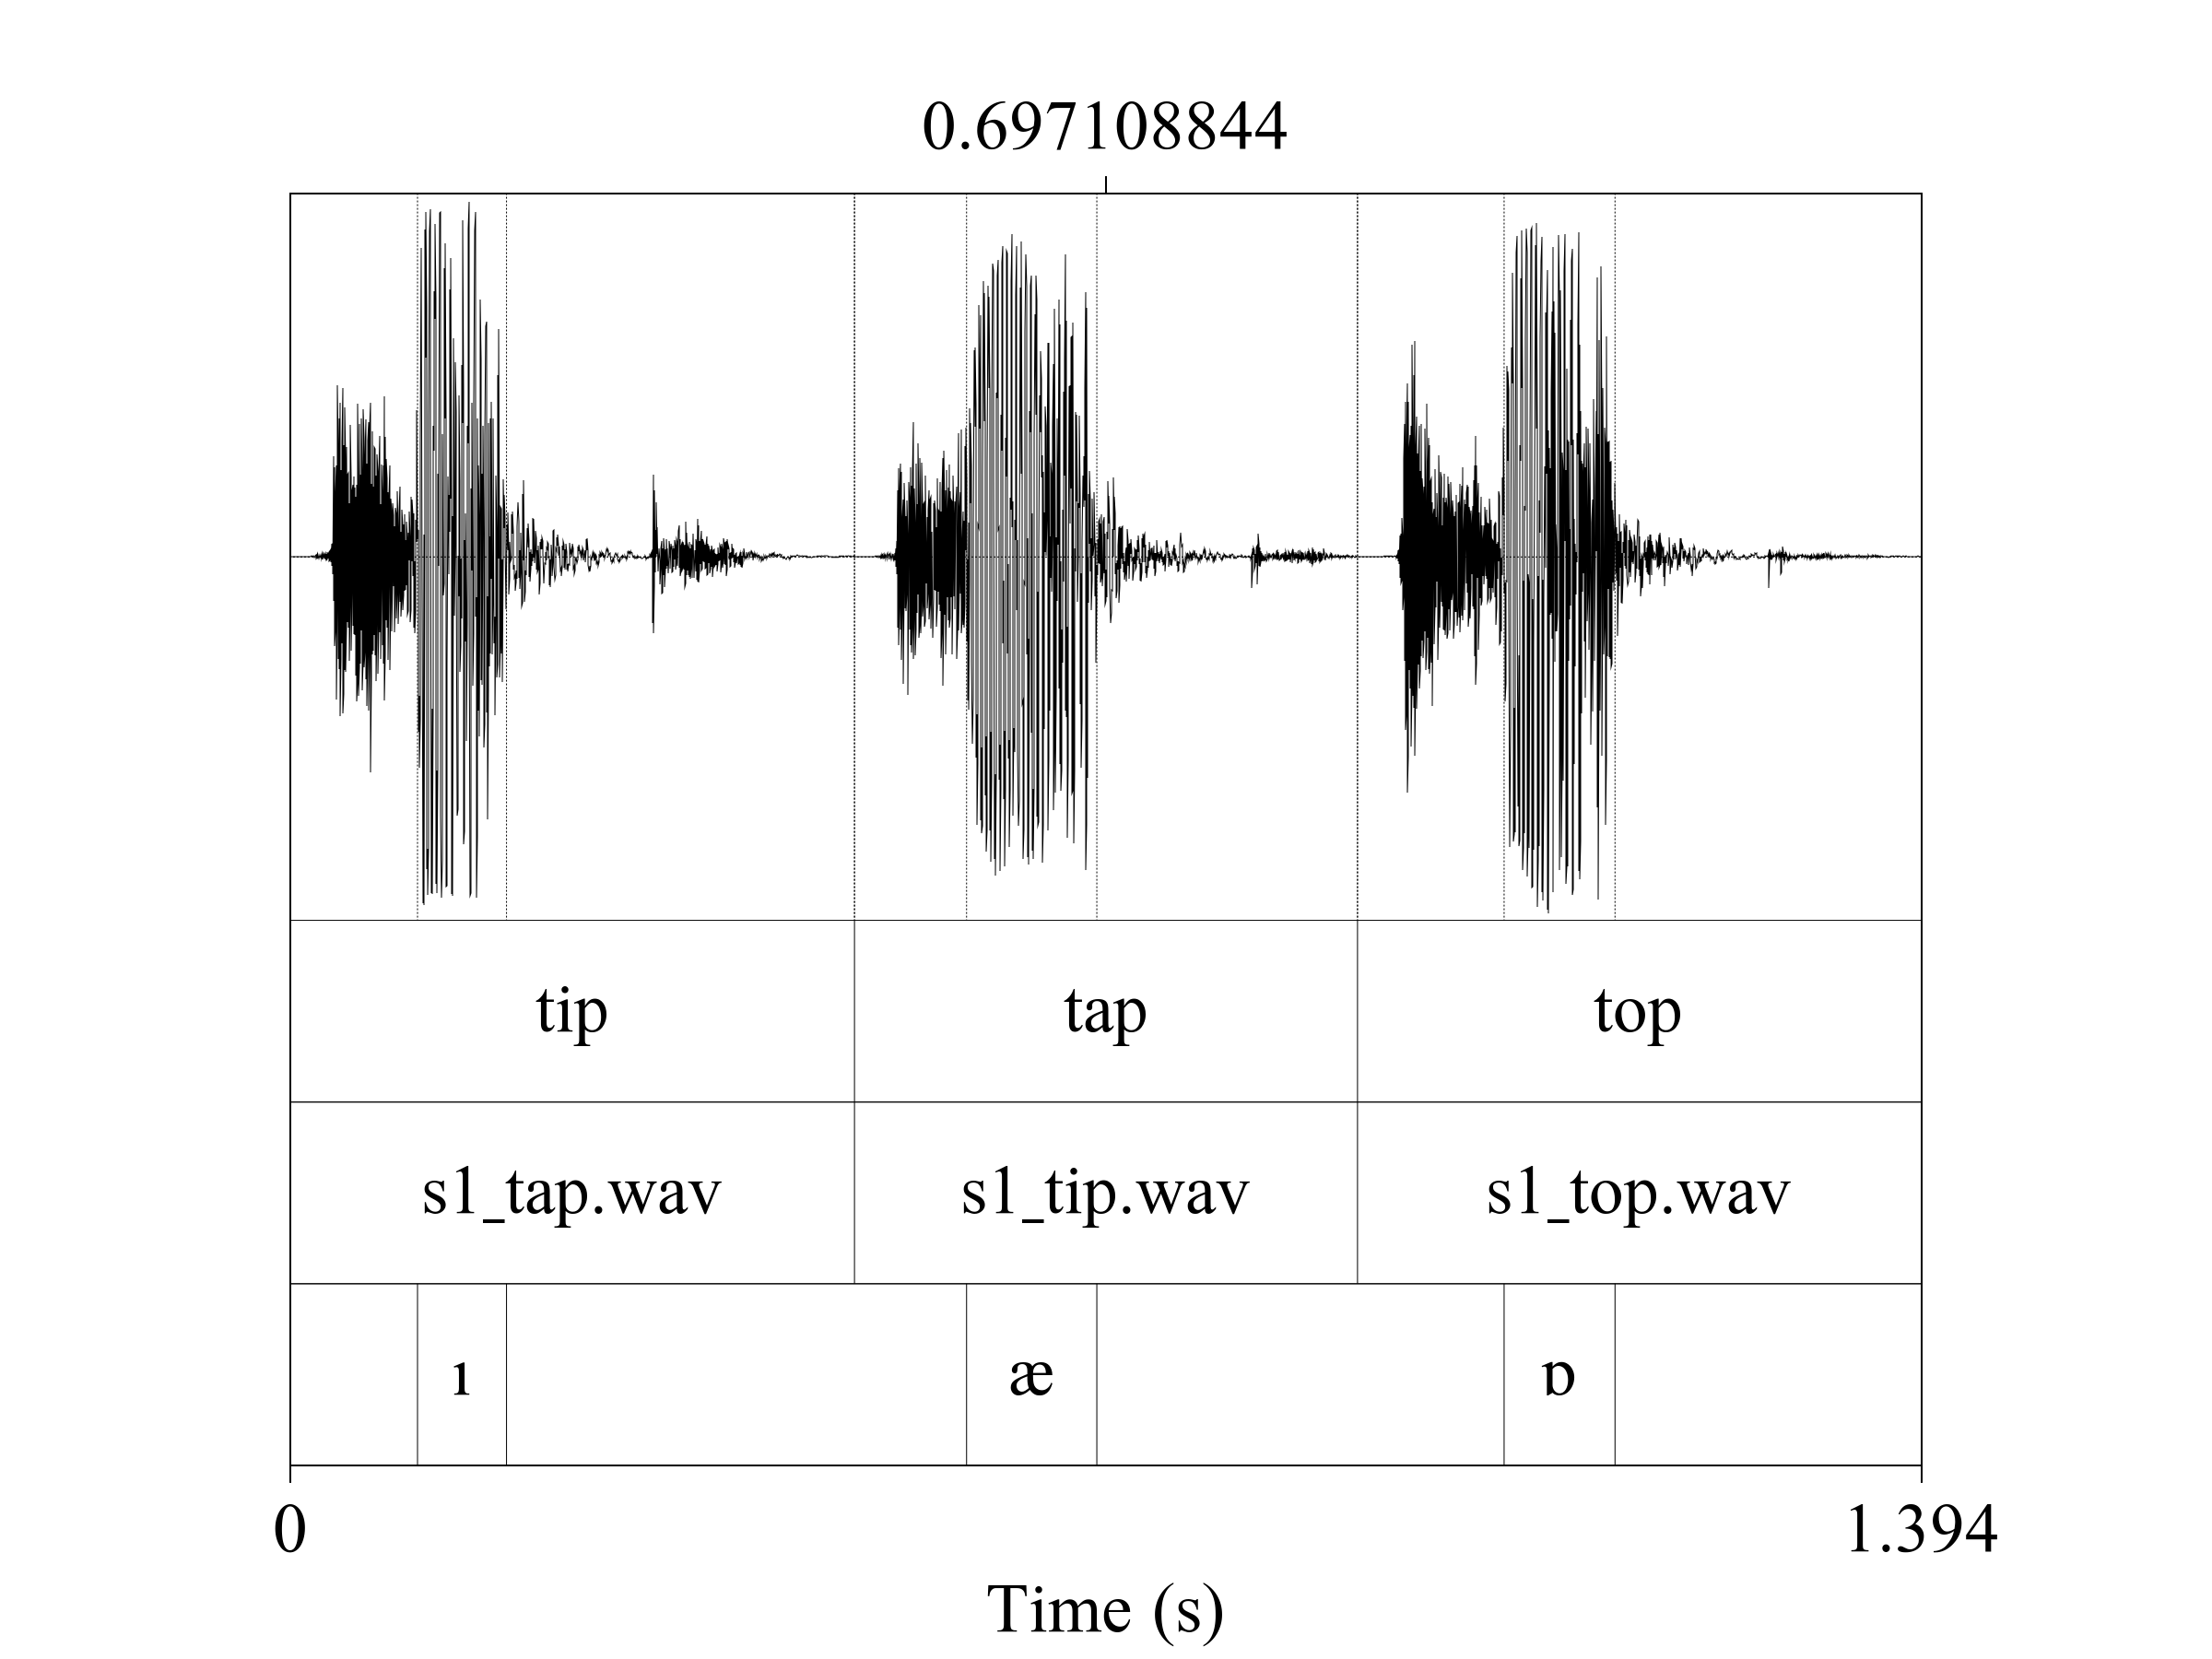
\includegraphics[width=0.7\linewidth]{images/06_annotate.png}
\end{frame}

\begin{frame}[fragile]{Automatically annotate your data}
Why should anybody separately annotate borders and fill gathered annotations with text?

I've participated in several projects with human annotations: there are a lot of typos. So this approach allow

\begin{itemize}
\item to avoid typographical problems; \pause
\item even if you don't like it, it is possible to automatically annotate words, translations, utterances etc.
\end{itemize} 
\end{frame}

\begin{frame}[fragile]{Extract annotated fragments}
Let's create a folder where all of the extracted files will be stored:
\begin{verbatim}
dir.create("s1/s1_sounds")
## │   ├── s1_all.TextGrid
## │   ├── s1_all.wav
## │   ├── s1_sounds     ←     we created this folder!
## │   ├── s1_tap.wav
## │   ├── s1_tip.wav
## │   └── s1_top.wav
## └── s2
##     ├──,,,
\end{verbatim}
\end{frame}

\begin{frame}[fragile]{Extract annotated fragments}
Let's create a folder where all of the extracted files will be stored:
\begin{verbatim}
extract_intervals(file_name = "s1/s1_all.wav", 
                  textgrid = "s1/s1_all.TextGrid",
                  tier = 3,
                  path = "s1/s1_sounds/",
                  prefix = "s1_")
## │   ├── s1_all.TextGrid
## │   ├── s1_all.wav
## │   ├── s1_sounds
## │   │   ├── 1_s1_ı.wav
## │   │   ├── 2_s1_æ.wav
## │   │   └── 3_s1_ɒ.wav
## │   ├── s1_tap.wav
## │   ├── s1_tip.wav
## │   └── s1_top.wav
## └── s2
##     ├──,,,
\end{verbatim}
\end{frame}

\begin{frame}[fragile]{Visualizing your data}
\begin{verbatim}
draw_sound(file_name = "s1/s1_sounds/1_s1_ı.wav")
\end{verbatim}
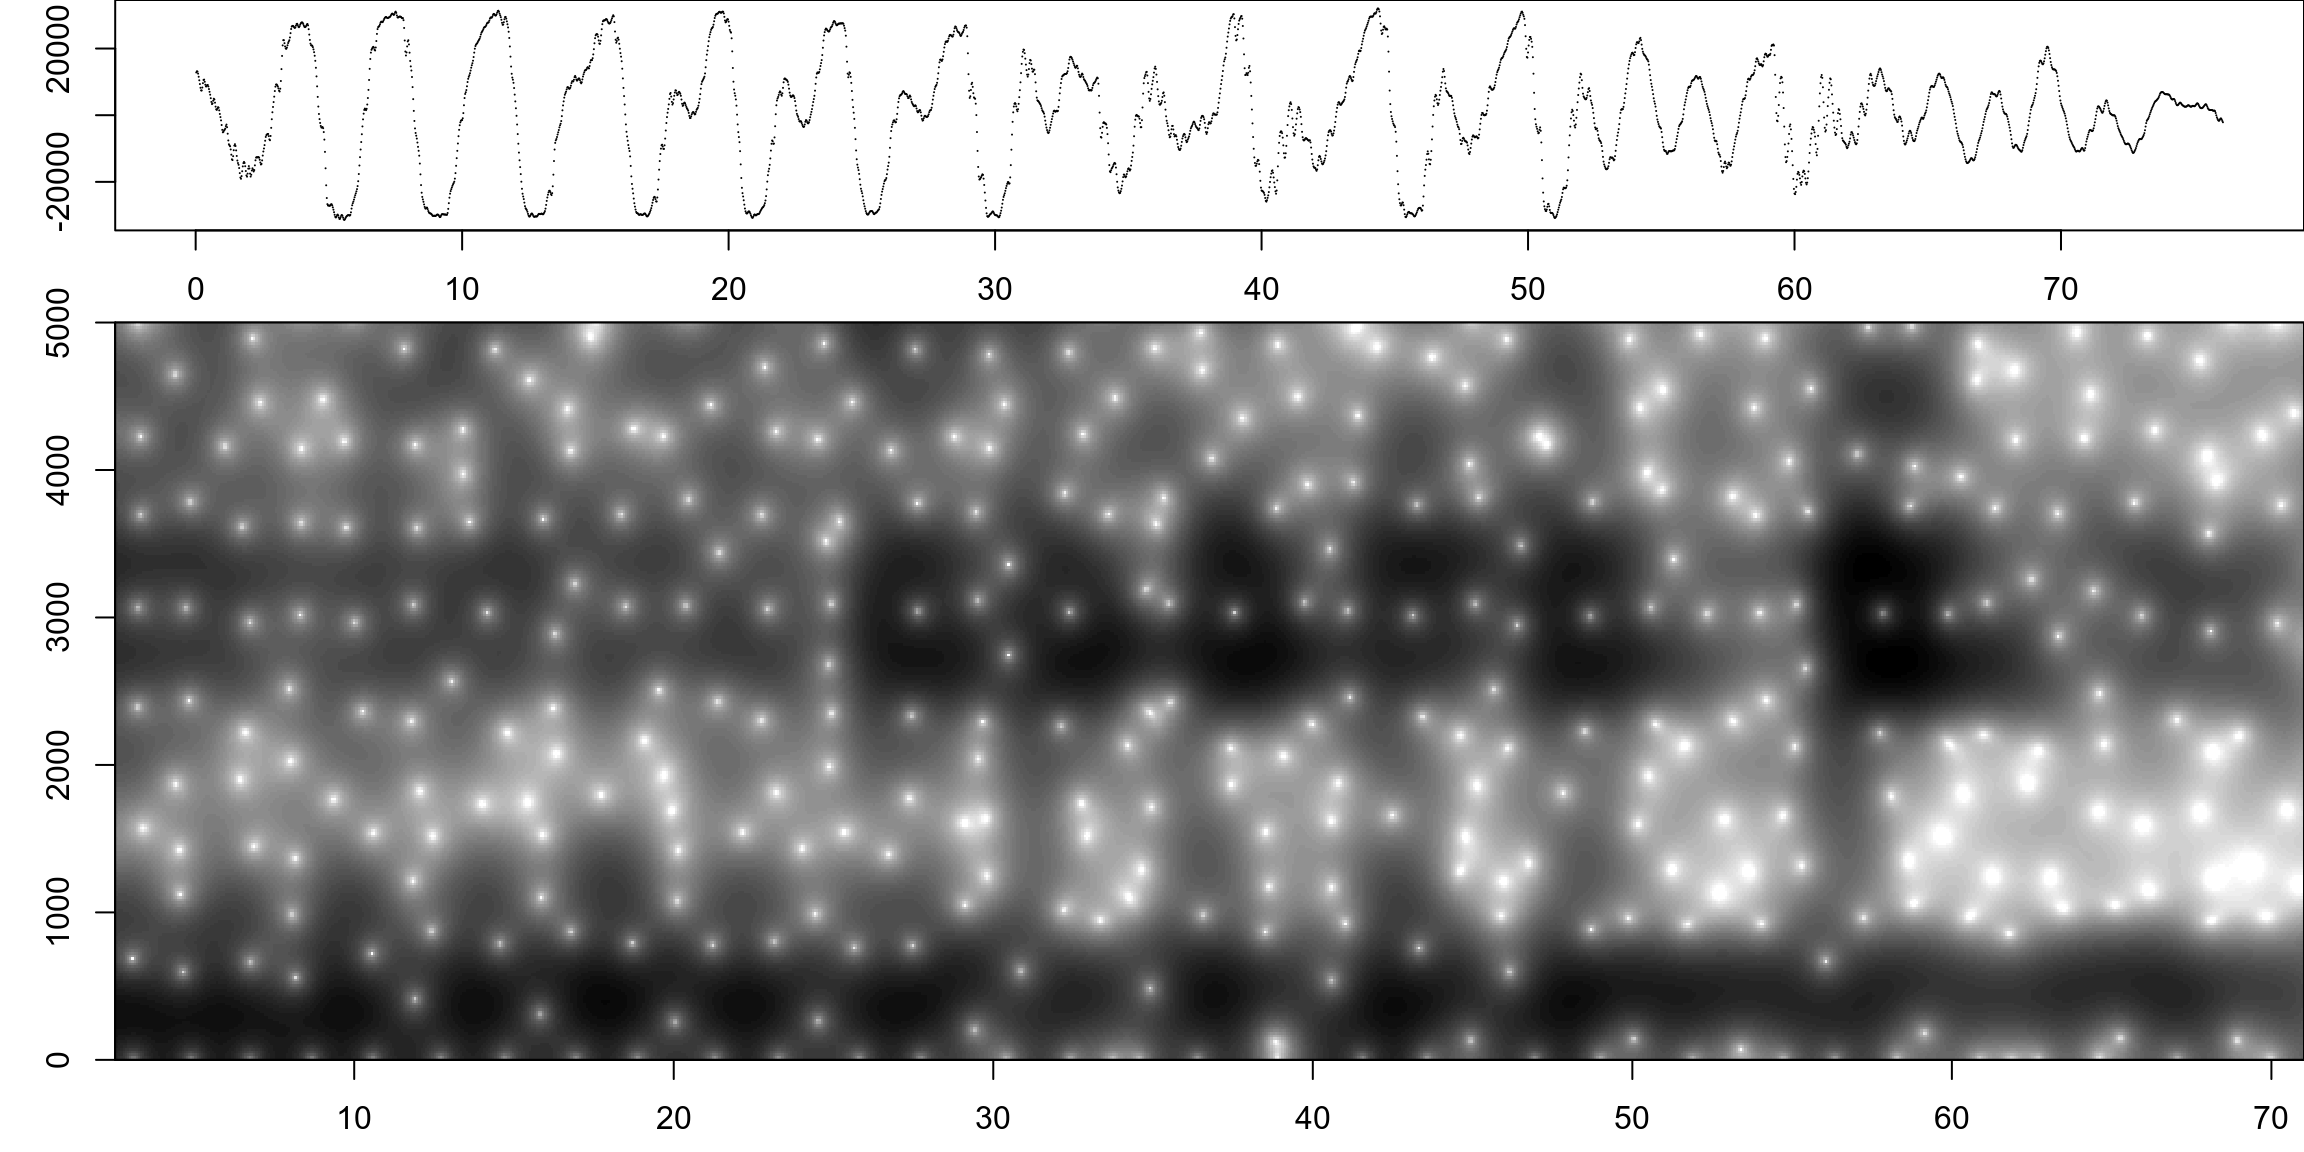
\includegraphics[width=\linewidth]{images/07_draw_sound.png}
\end{frame}

\begin{frame}[fragile]{Visualizing your data}
\begin{verbatim}
draw_sound(file_name = "s1/s1_sounds/1_s1_ı.wav")
\end{verbatim}
\begin{itemize}
\item \texttt{title} --- the title for the plot
\item \texttt{colores} --- set to (\texttt{TRUE}) for a colored spectogram, or (\texttt{FALSE}) for greyscale. It is also possible to provide a vector of custom colors for the spectrogram
\item \texttt{maximum\_frequency} --- the maximum frequency to be displayed for the spectrogram
\item \texttt{dynamic\_range} --- values greater than this many dB below the maximum will be displayed in the same color
\item \texttt{window\_length } --- the desired length in milliseconds for the analysis window
\item \texttt{output\_file} --- the name of the output file
\item \texttt{output\_width} --- the width of the device
\item \texttt{output\_height} --- the height of the device
\item \texttt{output\_units} --- the units in which height and width are given. This can be \texttt{"px"} (pixels, default), \texttt{"in"} (inches), \texttt{"cm"} or \texttt{"mm"}
\end{itemize}
\end{frame}

\begin{frame}[fragile]{Visualizing your data}
\begin{verbatim}
draw_sound(file_name = "s1/s1_sounds/1_s1_ı.wav", output_file = "s1/s1_tip", title = "s1 tip")
## ├── s1
## │   ├── s1_all.TextGrid
## │   ├── s1_all.wav
## │   ├── s1_sounds
## │   │   ├── 1_s1_ı.wav
## │   │   ├── 2_s1_æ.wav
## │   │   └── 3_s1_ɒ.wav
## │   ├── s1_tap.wav
## │   ├── s1_tip.png
## │   ├── s1_tip.wav
## │   └── s1_top.wav
## └── s2
## ...
\end{verbatim}
\end{frame}

\begin{frame}[fragile]{Visualizing your data}
\begin{verbatim}
draw_sound(sounds_from_folder = "s1/s1_sounds/", pic_folder_name = "s1_pics")
## ├── s1
## │   ├── s1_all.TextGrid
## │   ├── s1_all.wav
## │   ├── s1_pics
## │   │   ├── 1_s1_ı.png
## │   │   ├── 2_s1_æ.png
## │   │   └── 3_s1_ɒ.png
## │   ├── s1_sounds
## │   │   ├── 1_s1_ı.wav
## │   │   ├── 2_s1_æ.wav
## │   │   └── 3_s1_ɒ.wav
## │   ├── s1_tap.wav
## │   ├── s1_tip.png
## │   ├── s1_tip.wav
## │   └── s1_top.wav
## └── s2
##     ├── ...
\end{verbatim}
\end{frame}

\begin{frame}[fragile]{Create an \texttt{.html} viewer}
\begin{verbatim}
create_viewer(audio_dir = "s1/s1_sounds/",
              picture_dir = "s1/s1_pics/", 
              textgrid = "s1/s1_all.TextGrid",
              tiers = c(1, 3),
              output_dir = "s1/",
              output_file = "stimuli_viewer")
\end{verbatim}
\begin{itemize}
\item \href{https://agricolamz.github.io/phonfieldwork/s1/stimuli_viewer.html}{example 1}
\item \href{https://lingconlab.github.io/soqotri_emphatics/create_html.html}{example 2: Soqotri emphatics (Vasilisa Zhigulskaya's data)}
\end{itemize}
\end{frame}

\begin{frame}[fragile]{Cite the package}
\begin{verbatim}
citation("phonfieldwork")
## 
## Moroz G (2019). _Phonetic fieldwork and experiments with
## phonfieldwork package_. <URL:
## https://CRAN.R-project.org/package=phonfieldwork>.
## 
## A BibTeX entry for LaTeX users is
## 
##   @Manual{,
##     title = {Phonetic fieldwork and experiments with phonfieldwork package},
##     author = {George Moroz},
##     year = {2019},
##     url = {https://CRAN.R-project.org/package=phonfieldwork},
##   }
\end{verbatim}
\end{frame}

\framecard[colorblue]{{\color{colorwhite} \Large Send me a letter!\\
agricolamz@gmail.com\\ 
\vfill Presentation is available here: \\tinyurl.com/y3wtkcbq\\
\vfill 
\includegraphics[height = 4cm]{images/02_qrcode}}}

\begin{frame}{References}
\footnotesize
\bibliographystyle{config/chicago}
\bibliography{bibliography}
\end{frame}

\end{document}
